\chapter*{Purpose and use of this book}

{\small

\section*{Purpose}

This book is my attempt to present the text of the Iliad in an innovative format
for English speakers who are at an intermediate level in reading ancient Greek.
The goal is to have a paper version that you can read while sitting on the couch
with your terrier, without having to frequently consult a dictionary.

\section*{Layout}

Below is a photo mockup of the
idea. We have about 18 lines of Homer, in a large font, on a left-hand
page. There are aids surrounding this page: one page preceding it and
two pages following.

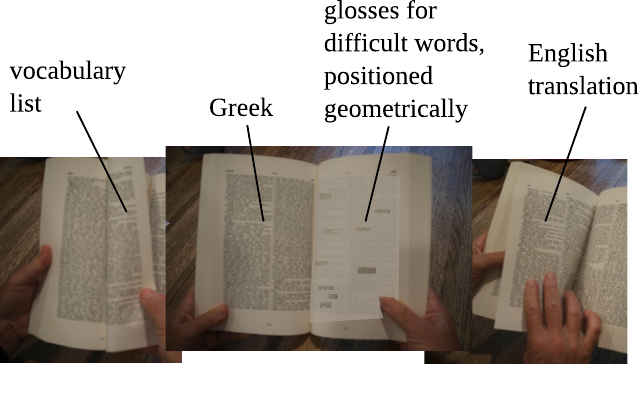
\includegraphics{iliad/figs/manual}

In this four-page sequence, the first page is a vocabulary list. It
contains every dictionary form (lemma) corresponding to the inflected
forms in the Greek text, except for a small core vocabulary (pp.~\pageref{core-vocab}-\pageref{core-vocab-end}).
It also lists a few inflections that may be difficult to recognize, such as irregular
aorists and some third-declension nouns.
The idea is that you may want to scan the vocabulary
list before you try to read the actual text, locking some of the less
common words into your short-term memory and priming your brain to
recognize inflected forms.

Next you turn the page and you have a two-page spread, in which the
left-hand page is Homer, and the right-hand page is the ``ransom note.''
The idea of the ransom note is that for the ten or twelve least common
words in the text, a translation is provided at a location that is at
the same geometrical position as the corresponding Greek word in the
actual text. These glosses are superimposed on top of a very light
gray copy of the actual text, to make it easier to see where the lines
lie and where the translation sits on its line. These words have also
already been listed on the vocab page. A reader who is highly
proficient and doesn't need much help may find that these words are
all they need, and they never need to look at the vocab page.

Finally, the fourth page is the English translation by Buckley, which you can flip to for help.

\section*{What this book is not}

This is not an introduction to ancient Greek for beginners, and it isn't a grammar textbook.
Absolute beginners may want to look at introductory books that were written using the Homeric
dialect, the best known text of this type being Pharr, Homeric Greek: A book for beginners.

This is not a substitute for a dictionary or a way to learn all the vocabulary for the first
time. The format I'm using here only allows enough space
for very brief \emph{reminder} of the basic definition of a word that you've already learned,
or an indication that you \emph{need} to learn certain words using a dictionary. For example,
the first word of the Iliad is μῆνις, which is glossed simply as ``rage.'' You will need a
dictionary to learn that it's feminine, that its genitive is μήνιος, and what are its connotations
and shades of meaning. Many of my glosses are abbreviated from Cunliffe (1924) or the English wiktionary, or in a few cases taken verbatim.

}
